\epigraph{Die Raumzeit ist fast dreidimensional. Aber \enquote{fast} macht den Unterschied.}{}

\section{Das Problem}


\begin{figure}[htbp]
\centering
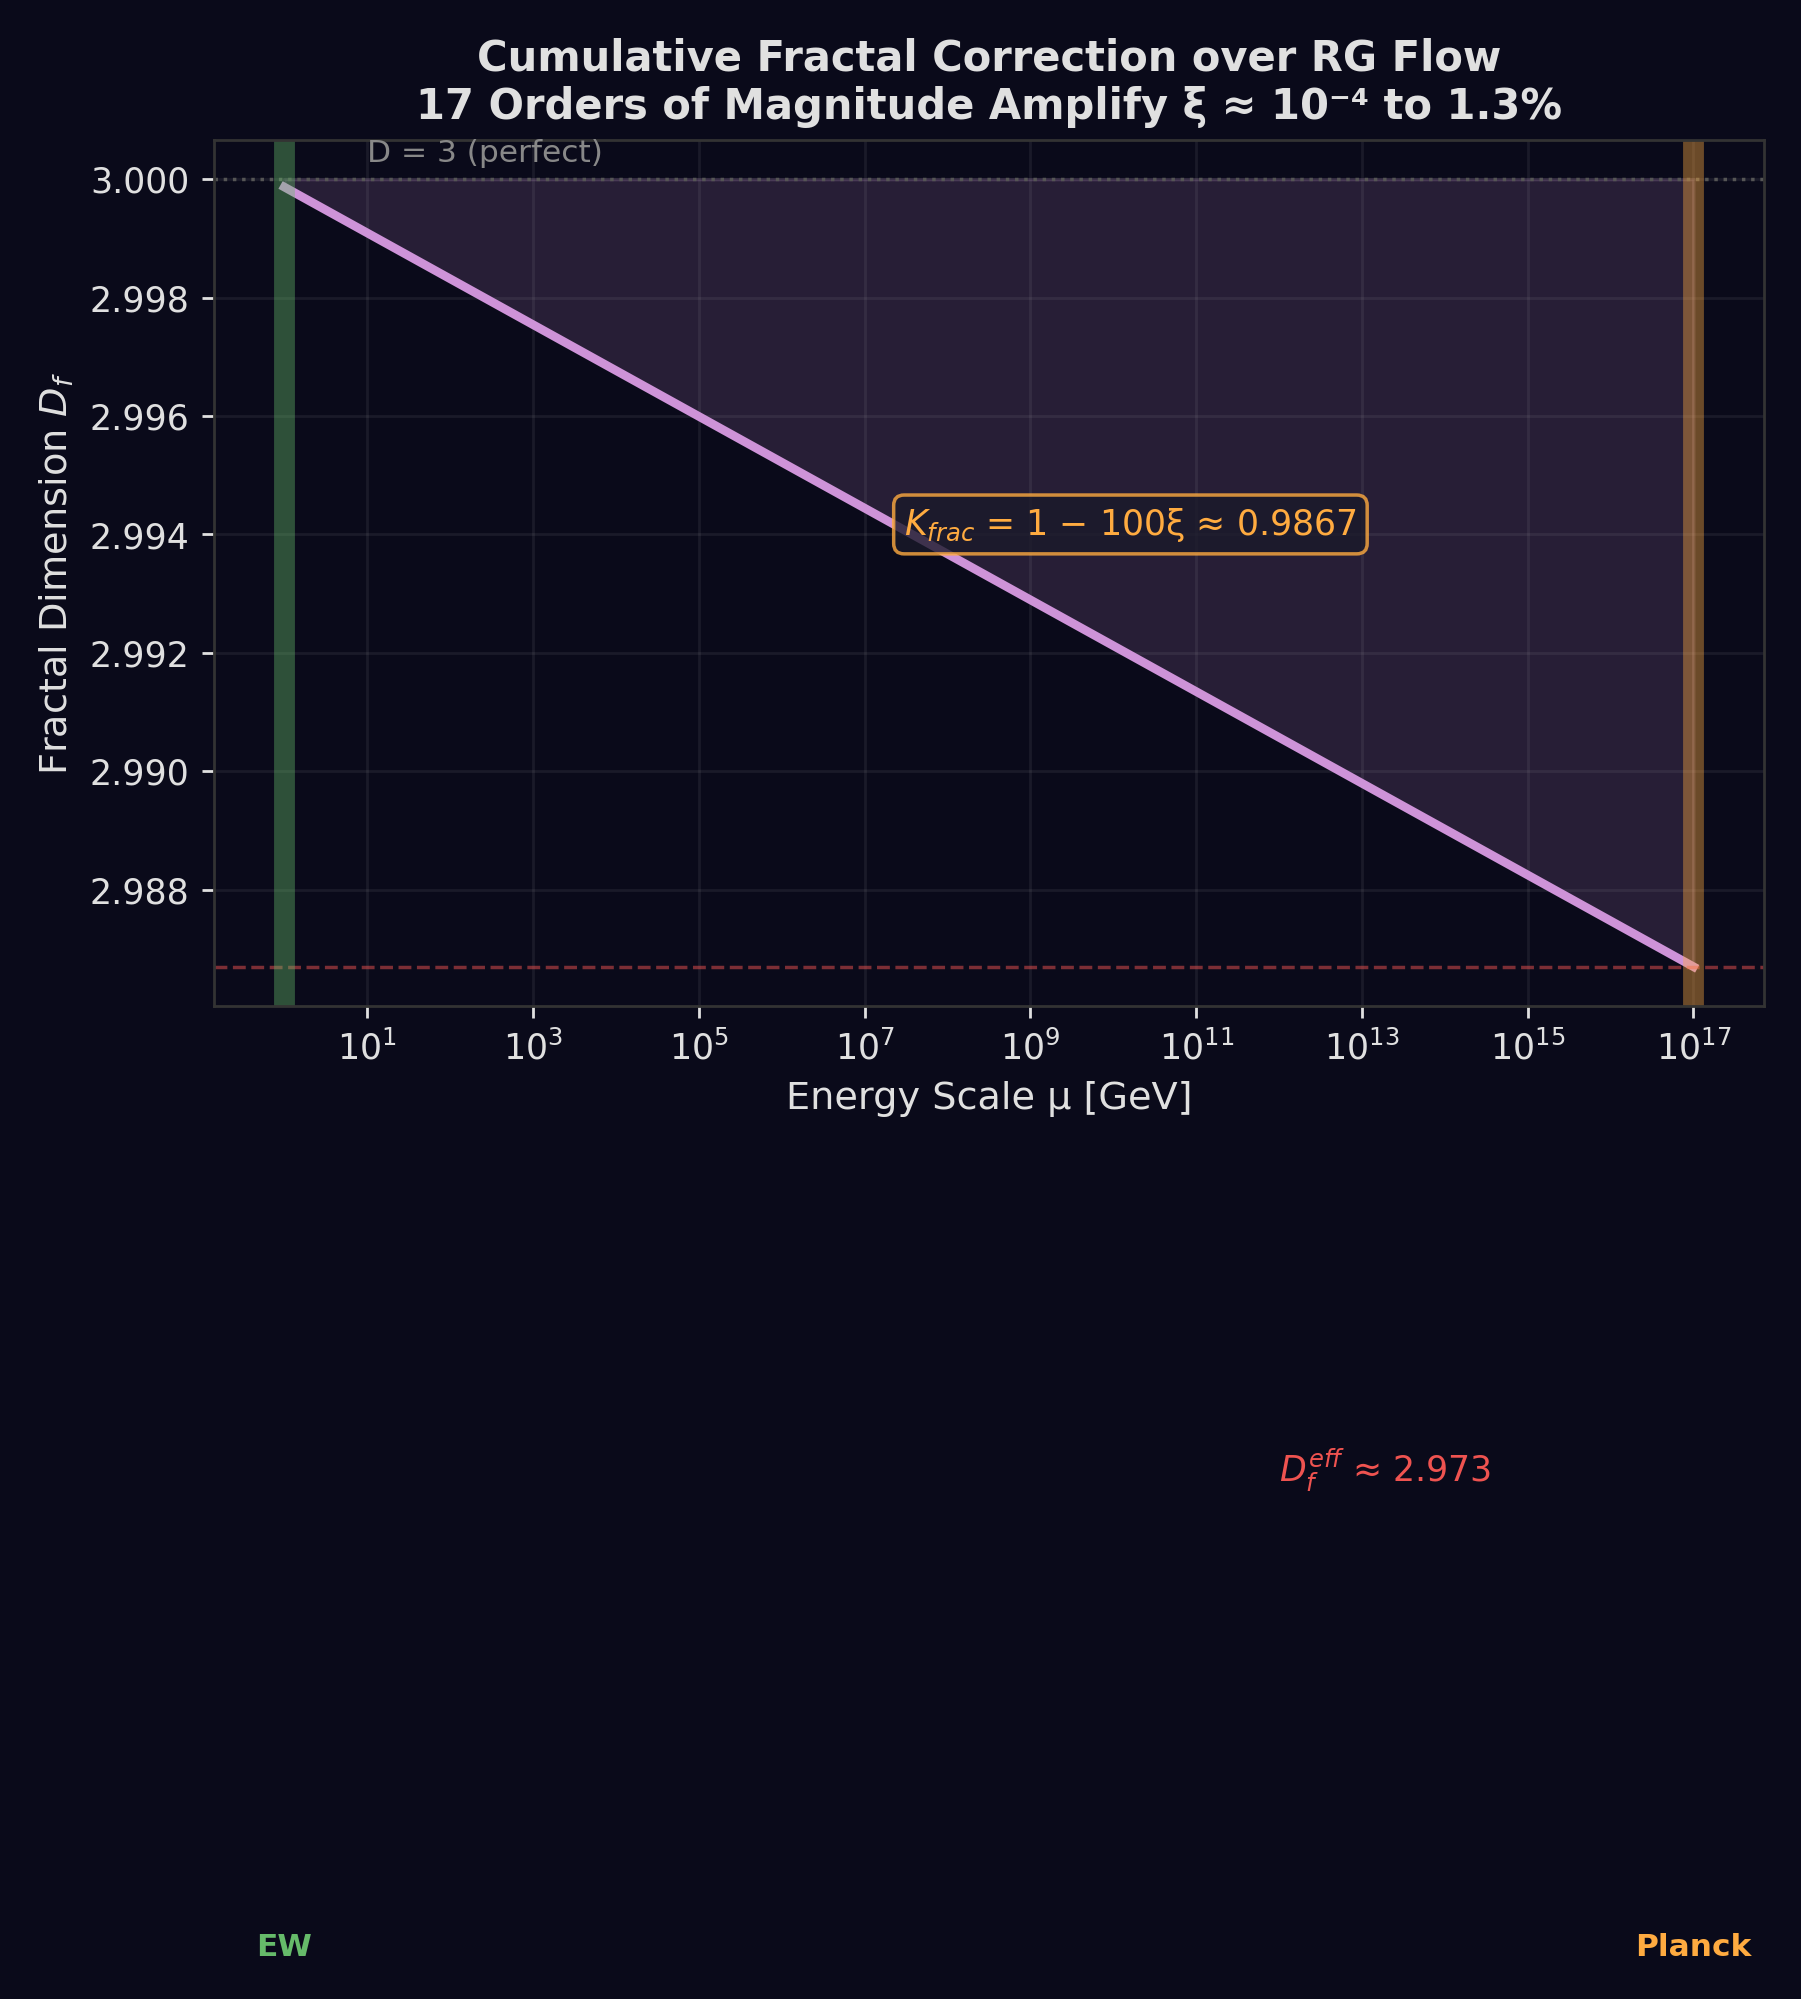
\includegraphics[width=0.85\textwidth]{img/ch09_fractal_rg.png}
\caption{Die kumulative fraktale Korrektur über den RG-Lauf von der EW- zur Planck-Skala.}
\end{figure}
Die Raumzeit ist nicht perfekt dreidimensional. Ihre lokale fraktale Dimension beträgt:
\begin{equation}
\Df^{\,\text{Raum}} = 3 - \xsi \approx 2{,}9998667
\end{equation}

Das ist eine winzige Abweichung --- nur~$\xsi \approx 1{,}33 \times 10^{-4}$ von der perfekten Drei. Und doch hat diese minimale Abweichung dramatische Konsequenzen.

\section{Zwei fraktale Dimensionen}

Ein subtiler, aber entscheidender Punkt: In der T0-Theorie treten \emph{zwei verschiedene} fraktale Dimensionen auf, die nicht verwechselt werden dürfen.

\subsection{Die Raumzeit-Dimension $\Df^{\,\text{Raum}} = 3 - \xsi$}

Die lokale Dimension der Raumzeit weicht nur minimal von~3 ab. Diese Abweichung beschreibt die \enquote{Porosität} der Raumzeit auf fundamentaler Ebene --- die Tatsache, dass die Kristallstruktur des Torus nicht perfekt dreidimensional packt.

Direkt eingesetzt in Volumenskalierungen liefert $\Df^{\,\text{Raum}} = 2{,}9999$ nur eine verschwindend kleine Korrektur: $(2{,}9999/3)^{2{,}9999/2} \approx 0{,}99993$ --- praktisch Eins.

\subsection{Die effektive Dimension und der RG-Lauf}

Die physikalisch relevante Korrektur entsteht nicht aus der lokalen Dimension allein, sondern aus der \emph{kumulativen Wirkung} dieser minimalen Abweichung über den gesamten Energiebereich von der Planck-Skala bis zur elektroschwachen Skala. Der Renormierungsgruppen-Lauf verstärkt die winzige lokale Abweichung~$\xsi$ zu einer messbaren Korrektur.

Der logarithmische Abstand zwischen den Skalen beträgt:
\begin{equation}
\ln\!\left(\frac{\ell_{\text{EW}}}{\lP}\right) \approx \ln(10^{17}) \approx 39
\end{equation}

Aus diesem Lauf und der geometrischen Mittelung über die relevanten Skalen entsteht ein effektiver Verstärkungsfaktor von~100. Die kumulative fraktale Korrektur ist daher nicht~$\xsi$, sondern~$100\xsi \approx 0{,}0133$, also rund~$1{,}3\%$.

\section{Der fraktale Korrekturfaktor}

Der physikalische Korrekturfaktor lautet:
\begin{equation}
\Kfrak = 1 - 100\xsi \approx 0{,}9867
\end{equation}

Dies lässt sich äquivalent als Potenzformel schreiben:
\begin{equation}
\Kfrak = \left(\frac{\Df^{\,\text{eff}}}{3}\right)^{\!\Df^{\,\text{eff}}/2} \qquad \text{mit } \Df^{\,\text{eff}} \approx 2{,}973
\end{equation}

Die effektive Dimension~$\Df^{\,\text{eff}} \approx 2{,}973$ ist nicht identisch mit der Raumzeit-Dimension~$\Df^{\,\text{Raum}} = 2{,}9999$. Sie beschreibt die \emph{kumulative} Wirkung der fraktalen Struktur auf die Massendynamik über den gesamten RG-Lauf. Die Raumzeit weicht lokal kaum von~3 ab, aber über 17~Größenordnungen Energielauf akkumuliert sich die Abweichung zu einer messbaren~$1{,}3\%$-Korrektur.

Alternativ lässt sich $\Kfrak$ aus dem Renormierungsgruppen-Integral ableiten (vgl.\ \href{https://github.com/jpascher/T0-Time-Mass-Duality/blob/main/2/pdf/133_Fraktale_Korrektur_Herleitung_De.pdf}{Dok.~133}):
\begin{equation}
\Kfrak = \exp\!\left(-\int_{\mu_{\text{EW}}}^{\mu_P} \frac{\gamma(\mu)}{\mu}\,d\mu\right) \approx 1 - 100\xsi
\end{equation}
wobei~$\gamma(\mu)$ die anomale Dimension des Massenfeldes ist.

\begin{kerngedanke}
Die scheinbar willkürliche Zahl~100 in $\Kfrak = 1 - 100\xsi$ hat eine präzise physikalische Herkunft: Sie beschreibt die kumulative Wirkung der fraktalen Raumzeitstruktur über den Renormierungsgruppen-Lauf von der Planck-Skala zur elektroschwachen Skala. Eine winzige lokale Abweichung ($\xsi \approx 10^{-4}$) wird durch 17~Größenordnungen Energielauf zu einer messbaren Korrektur verstärkt.
\end{kerngedanke}

\section{Warum $\Kfrak$ notwendig ist --- der Eindeutigkeitsbeweis}

Die Notwendigkeit von~$\Kfrak$ lässt sich durch einen eleganten Konsistenzbeweis zeigen (\href{https://github.com/jpascher/T0-Time-Mass-Duality/blob/main/2/pdf/133_Fraktale_Korrektur_Herleitung_De.pdf}{Dok.~133}). Es gibt zwei unabhängige Wege, das Massenverhältnis~$m_e/m_\mu$ zu berechnen:

\textbf{Weg~1 (fraktal):} Aus der T0-Geometrie mit fraktaler Integration folgen Massenformeln der Form $m_e \propto \xsi^{5/2}$ und $m_\mu \propto \xsi^2$, wobei die Koeffizienten von der effektiven fraktalen Dimension abhängen.

\textbf{Weg~2 (direkt):} Aus der reinen tetraedrischen Symmetrie ohne fraktale Korrekturen folgt ein unabhängiger Ausdruck für $m_e/m_\mu$.

Die Forderung, dass beide Wege denselben experimentellen Wert liefern, bestimmt~$\Df^{\,\text{eff}}$ \emph{eindeutig}. Es gibt genau einen Wert, der konsistent ist --- und dieser liefert $\Kfrak = 1 - 100\xsi \approx 0{,}9867$.

$\Kfrak$ ist damit keine freie Wahl, kein Anpassungsparameter. Er ist eine geometrische Notwendigkeit, erzwungen durch die innere Konsistenz der Theorie.

\section{Wann braucht man $\Kfrak$ --- und wann nicht?}

Die Korrektur ist \textbf{nicht nötig} für Massenverhältnisse, Energieverhältnisse und dimensionslose Kopplungskonstanten. In Verhältnissen kürzt sich der Faktor heraus --- ein weiterer Hinweis darauf, dass Verhältnisse fundamentaler sind als absolute Werte.

Sie ist \textbf{nötig} für absolute Massen in SI-Einheiten, für die Feinstrukturkonstante berechnet aus Massen und für Kopplungen an externe Felder.

\section{Die tiefere Bedeutung}

Hinter der Korrektur $\Kfrak$ verbirgt sich eine Einsicht von großer Tragweite. In einer Raumzeit mit $\Df < 3$ haben Pfadintegrale weniger verfügbare Pfade als in exakt drei Dimensionen. Propagatoren erhalten einen zusätzlichen Dämpfungsfaktor. Volumina und Flächen sind leicht kleiner als in perfekt dreidimensionalem Raum.

Die fraktale Raumzeit wirkt wie ein natürlicher Regulator. Die Divergenzen, die in der Standard-QFT durch aufwendige Renormierung gebändigt werden müssen, entstehen in T0 gar nicht erst --- weil die Raumzeit selbst einen eingebauten Cutoff besitzt.

\begin{zusammenfassung}
Die fraktale Korrektur~$\Kfrak = 1 - 100\xsi \approx 0{,}9867$ entsteht nicht aus der lokalen Raumzeit-Dimension allein ($\Df^{\,\text{Raum}} = 3 - \xsi \approx 2{,}9999$), sondern aus der \emph{kumulativen Wirkung} dieser Abweichung über den RG-Lauf von der Planck- zur elektroschwachen Skala. Die äquivalente Potenzformel $(\Df^{\,\text{eff}}/3)^{\Df^{\,\text{eff}}/2}$ mit $\Df^{\,\text{eff}} \approx 2{,}97$ beschreibt diese kumulative Wirkung. Der Faktor ist keine Zusatzannahme, sondern folgt zwingend aus der Konsistenz zweier unabhängiger Herleitungswege.
\end{zusammenfassung}
